\section{Miscellaneous Image Transformations}

\ifCPy

\cvCPyFunc{AdaptiveThreshold}
Applies an adaptive threshold to an array.

\cvdefC{
void cvAdaptiveThreshold(
\par const CvArr* src,\par CvArr* dst,\par double maxValue,\par
int adaptive\_method=CV\_ADAPTIVE\_THRESH\_MEAN\_C,\par
int thresholdType=CV\_THRESH\_BINARY,\par
int blockSize=3,\par double param1=5 );
}

\cvdefPy{AdaptiveThreshold(src,dst,maxValue, adaptive\_method=CV\_ADAPTIVE\_THRESH\_MEAN\_C, thresholdType=CV\_THRESH\_BINARY,blockSize=3,param1=5)-> None}

\begin{description}
\cvarg{src}{Source image}
\cvarg{dst}{Destination image}
\cvarg{maxValue}{Maximum value that is used with \texttt{CV\_THRESH\_BINARY} and \texttt{CV\_THRESH\_BINARY\_INV}}
\cvarg{adaptive\_method}{Adaptive thresholding algorithm to use: \texttt{CV\_ADAPTIVE\_THRESH\_MEAN\_C} or \texttt{CV\_ADAPTIVE\_THRESH\_GAUSSIAN\_C} (see the discussion)}
\cvarg{thresholdType}{Thresholding type; must be one of
\begin{description}
  \cvarg{CV\_THRESH\_BINARY}{xxx}
  \cvarg{CV\_THRESH\_BINARY\_INV}{xxx}
\end{description}}
\cvarg{blockSize}{The size of a pixel neighborhood that is used to calculate a threshold value for the pixel: 3, 5, 7, and so on}
\cvarg{param1}{The method-dependent parameter. For the methods \texttt{CV\_ADAPTIVE\_THRESH\_MEAN\_C} and \texttt{CV\_ADAPTIVE\_THRESH\_GAUSSIAN\_C} it is a constant subtracted from the mean or weighted mean (see the discussion), though it may be negative}
\end{description}

The function transforms a grayscale image to a binary image according to the formulas:

\begin{description}
\cvarg{CV\_THRESH\_BINARY}{\[ dst(x,y) = \fork{\texttt{maxValue}}{if $src(x,y) > T(x,y)$}{0}{otherwise} \]}
\cvarg{CV\_THRESH\_BINARY\_INV}{\[ dst(x,y) = \fork{0}{if $src(x,y) > T(x,y)$}{\texttt{maxValue}}{otherwise} \]}
\end{description}

where $T(x,y)$ is a threshold calculated individually for each pixel.

For the method \texttt{CV\_ADAPTIVE\_THRESH\_MEAN\_C} it is the mean of a $\texttt{blockSize} \times \texttt{blockSize}$ pixel neighborhood, minus \texttt{param1}.

For the method \texttt{CV\_ADAPTIVE\_THRESH\_GAUSSIAN\_C} it is the weighted sum (gaussian) of a $\texttt{blockSize} \times \texttt{blockSize}$ pixel neighborhood, minus \texttt{param1}.

\cvCPyFunc{CvtColor}
Converts an image from one color space to another.

\cvdefC{
void cvCvtColor(
\par const CvArr* src,
\par CvArr* dst,
\par int code );
}\cvdefPy{CvtColor(src,dst,code)-> None}

\begin{description}
\cvarg{src}{The source 8-bit (8u), 16-bit (16u) or single-precision floating-point (32f) image}
\cvarg{dst}{The destination image of the same data type as the source. The number of channels may be different}
\cvarg{code}{Color conversion operation that can be specifed using \texttt{CV\_ \textit{src\_color\_space} 2 \textit{dst\_color\_space}} constants (see below)}
\end{description}

The function converts the input image from one color
space to another. The function ignores the \texttt{colorModel} and
\texttt{channelSeq} fields of the \texttt{IplImage} header, so the
source image color space should be specified correctly (including
order of the channels in the case of RGB space. For example, BGR means 24-bit
format with $B_0, G_0, R_0, B_1, G_1, R_1, ...$ layout
whereas RGB means 24-format with $R_0, G_0, B_0, R_1, G_1, B_1, ...$
layout).

The conventional range for R,G,B channel values is:

\begin{itemize}
 \item 0 to 255 for 8-bit images
 \item 0 to 65535 for 16-bit images and
 \item 0 to 1 for floating-point images.
\end{itemize}

Of course, in the case of linear transformations the range can be
specific, but in order to get correct results in the case of non-linear
transformations, the input image should be scaled.

The function can do the following transformations:

\begin{itemize}
 \item Transformations within RGB space like adding/removing the alpha channel, reversing the channel order, conversion to/from 16-bit RGB color (R5:G6:B5 or R5:G5:B5), as well as conversion to/from grayscale using:
 \[
 \text{RGB[A] to Gray:} Y \leftarrow 0.299 \cdot R + 0.587 \cdot G + 0.114 \cdot B
 \]
 and
 \[
 \text{Gray to RGB[A]:} R \leftarrow Y, G \leftarrow Y, B \leftarrow Y, A \leftarrow 0
 \]

The conversion from a RGB image to gray is done with:
\begin{lstlisting}
cvCvtColor(src ,bwsrc, CV_RGB2GRAY)
\end{lstlisting}

 \item RGB $\leftrightarrow$ CIE XYZ.Rec 709 with D65 white point (\texttt{CV\_BGR2XYZ, CV\_RGB2XYZ, CV\_XYZ2BGR, CV\_XYZ2RGB}):
 \[
 \begin{bmatrix}
 X \\
 Y \\
 Z
 \end{bmatrix}
 \leftarrow
 \begin{bmatrix}
0.412453 & 0.357580 & 0.180423\\
0.212671 & 0.715160 & 0.072169\\
0.019334 & 0.119193 & 0.950227
 \end{bmatrix}
 \cdot
 \begin{bmatrix}
 R \\
 G \\
 B
 \end{bmatrix}
 \]
 \[
 \begin{bmatrix}
 R \\
 G \\
 B
 \end{bmatrix}
 \leftarrow
 \begin{bmatrix}
3.240479 & -1.53715 & -0.498535\\
-0.969256 &  1.875991 & 0.041556\\
0.055648 & -0.204043 & 1.057311
 \end{bmatrix}
 \cdot
 \begin{bmatrix}
 X \\
 Y \\
 Z
 \end{bmatrix}
 \]
$X$, $Y$ and $Z$ cover the whole value range (in the case of floating-point images $Z$ may exceed 1).

 \item RGB $\leftrightarrow$ YCrCb JPEG (a.k.a. YCC) (\texttt{CV\_BGR2YCrCb, CV\_RGB2YCrCb, CV\_YCrCb2BGR, CV\_YCrCb2RGB})
 \[ Y \leftarrow 0.299 \cdot R + 0.587 \cdot G + 0.114 \cdot B \]
 \[  Cr \leftarrow (R-Y) \cdot 0.713 + delta \]
 \[  Cb \leftarrow (B-Y) \cdot 0.564 + delta \]
 \[  R \leftarrow Y + 1.403 \cdot (Cr - delta) \]
 \[  G \leftarrow Y - 0.344 \cdot (Cr - delta) - 0.714 \cdot (Cb - delta) \]
 \[  B \leftarrow Y + 1.773 \cdot (Cb - delta) \]
where
 \[
  delta = \left\{
  \begin{array}{l l}
  128 & \mbox{for 8-bit images}\\
  32768 & \mbox{for 16-bit images}\\
  0.5 & \mbox{for floating-point images}
  \end{array} \right.
 \]
Y, Cr and Cb cover the whole value range.

 \item RGB $\leftrightarrow$ HSV (\texttt{CV\_BGR2HSV, CV\_RGB2HSV, CV\_HSV2BGR, CV\_HSV2RGB})
  in the case of 8-bit and 16-bit images
  R, G and B are converted to floating-point format and scaled to fit the 0 to 1 range
  \[ V \leftarrow max(R,G,B) \]

\[ S \leftarrow \fork{\frac{V-min(R,G,B)}{V}}{if $V \neq 0$}{0}{otherwise} \]
\[ H \leftarrow \forkthree
{{60(G - B)}/{S}}{if $V=R$}
{{120+60(B - R)}/{S}}{if $V=G$}
{{240+60(R - G)}/{S}}{if $V=B$} \]
if $H<0$ then $H \leftarrow H+360$

On output $0 \leq V \leq 1$, $0 \leq S \leq 1$, $0 \leq H \leq 360$.

The values are then converted to the destination data type:
\begin{description}
\item[8-bit images]
\[ V \leftarrow 255 V, S \leftarrow 255 S, H \leftarrow H/2 \text{(to fit to 0 to 255)} \]
\item[16-bit images (currently not supported)]
\[ V <- 65535 V, S <- 65535 S, H <- H \]
\item[32-bit images]
H, S, V are left as is
\end{description}

 \item RGB $\leftrightarrow$ HLS (\texttt{CV\_BGR2HLS, CV\_RGB2HLS, CV\_HLS2BGR, CV\_HLS2RGB}).
  in the case of 8-bit and 16-bit images
  R, G and B are converted to floating-point format and scaled to fit the 0 to 1 range.
  \[ V_{max} \leftarrow {max}(R,G,B) \]
  \[ V_{min} \leftarrow {min}(R,G,B) \]
  \[ L \leftarrow \frac{V_{max} - V_{min}}{2} \]
  \[ S \leftarrow \fork
    {\frac{V_{max} - V_{min}}{V_{max} + V_{min}}}{if $L < 0.5$}
    {\frac{V_{max} - V_{min}}{2 - (V_{max} + V_{min})}}{if $L \ge 0.5$} \]
  \[ H \leftarrow \forkthree
  {{60(G - B)}/{S}}{if $V_{max}=R$}
  {{120+60(B - R)}/{S}}{if $V_{max}=G$}
  {{240+60(R - G)}/{S}}{if $V_{max}=B$} \]
  if $H<0$ then $H \leftarrow H+360$
On output $0 \leq V \leq 1$, $0 \leq S \leq 1$, $0 \leq H \leq 360$.

The values are then converted to the destination data type:
\begin{description}
\item[8-bit images]
\[ V \leftarrow 255 V, S \leftarrow 255 S, H \leftarrow H/2 \text{(to fit to 0 to 255)} \]
\item[16-bit images (currently not supported)]
\[ V <- 65535 V, S <- 65535 S, H <- H \]
\item[32-bit images]
H, S, V are left as is
\end{description}

 \item RGB $\leftrightarrow$ CIE L*a*b* (\texttt{CV\_BGR2Lab, CV\_RGB2Lab, CV\_Lab2BGR, CV\_Lab2RGB})
  in the case of 8-bit and 16-bit images
  R, G and B are converted to floating-point format and scaled to fit the 0 to 1 range
\[ \vecthree{X}{Y}{Z} \leftarrow \vecthreethree
{0.412453}{0.357580}{0.180423}
{0.212671}{0.715160}{0.072169}
{0.019334}{0.119193}{0.950227}
\cdot
\vecthree{R}{G}{B} \]
\[ X \leftarrow X/X_n, \text{where} X_n = 0.950456 \]
\[ Z \leftarrow Z/Z_n, \text{where} Z_n = 1.088754 \]
\[ L \leftarrow \fork
{116*Y^{1/3}-16}{for $Y>0.008856$}
{903.3*Y}{for $Y \le 0.008856$} \]
\[ a \leftarrow 500 (f(X)-f(Y)) + delta \]
\[ b \leftarrow 200 (f(Y)-f(Z)) + delta \]
where
\[f(t)=\fork
{t^{1/3}}{for $t>0.008856$}
{7.787 t+16/116}{for $t<=0.008856$} \]
and
\[ delta = \fork{128}{for 8-bit images}{0}{for floating-point images} \]
On output $0 \leq L \leq 100$, $-127 \leq a \leq 127$, $-127 \leq b \leq 127$

The values are then converted to the destination data type:
\begin{description}
\item[8-bit images]
\[L \leftarrow L*255/100, a \leftarrow a + 128, b \leftarrow b + 128\]
\item[16-bit images] currently not supported
\item[32-bit images]
L, a, b are left as is
\end{description}

 \item RGB $\leftrightarrow$ CIE L*u*v* (\texttt{CV\_BGR2Luv, CV\_RGB2Luv, CV\_Luv2BGR, CV\_Luv2RGB})
  in the case of 8-bit and 16-bit images
  R, G and B are converted to floating-point format and scaled to fit 0 to 1 range
  \[ \vecthree{X}{Y}{Z} \leftarrow \vecthreethree
{0.412453}{0.357580}{0.180423}
{0.212671}{0.715160}{0.072169}
{0.019334}{0.119193}{0.950227}
\cdot
\vecthree{R}{G}{B} \]
\[ L \leftarrow \fork
{116 Y^{1/3}}{for $Y>0.008856$}
{903.3 Y}{for $Y<=0.008856$} \]
\[ u' \leftarrow 4*X/(X + 15*Y + 3 Z) \]
\[ v' \leftarrow 9*Y/(X + 15*Y + 3 Z) \]
\[ u \leftarrow 13*L*(u' - u_n) \quad \text{where} \quad u_n=0.19793943 \]
\[ v \leftarrow 13*L*(v' - v_n) \quad \text{where} \quad v_n=0.46831096 \]
On output $0 \leq L \leq 100$, $-134 \leq u \leq 220$, $-140 \leq v \leq 122$.

The values are then converted to the destination data type:
\begin{description}
\item[8-bit images]
\[L \leftarrow 255/100 L, u \leftarrow 255/354 (u + 134), v \leftarrow 255/256 (v + 140) \]
\item[16-bit images] currently not supported
\item[32-bit images] L, u, v are left as is
\end{description}

The above formulas for converting RGB to/from various color spaces have been taken from multiple sources on Web, primarily from
the Ford98
 at the Charles Poynton site.

 \item Bayer $\rightarrow$ RGB (\texttt{CV\_BayerBG2BGR, CV\_BayerGB2BGR, CV\_BayerRG2BGR, CV\_BayerGR2BGR, CV\_BayerBG2RGB, CV\_BayerGB2RGB, CV\_BayerRG2RGB, CV\_BayerGR2RGB}) The Bayer pattern is widely used in CCD and CMOS cameras. It allows one to get color pictures from a single plane where R,G and B pixels (sensors of a particular component) are interleaved like this:



\[
\newcommand{\Rcell}{\color{red}R}
\newcommand{\Gcell}{\color{green}G}
\newcommand{\Bcell}{\color{blue}B}
\definecolor{BackGray}{rgb}{0.8,0.8,0.8}
\begin{array}{ c c c c c }
\Rcell&\Gcell&\Rcell&\Gcell&\Rcell\\
\Gcell&\colorbox{BackGray}{\Bcell}&\colorbox{BackGray}{\Gcell}&\Bcell&\Gcell\\
\Rcell&\Gcell&\Rcell&\Gcell&\Rcell\\
\Gcell&\Bcell&\Gcell&\Bcell&\Gcell\\
\Rcell&\Gcell&\Rcell&\Gcell&\Rcell
\end{array}
\]

The output RGB components of a pixel are interpolated from 1, 2 or
4 neighbors of the pixel having the same color. There are several
modifications of the above pattern that can be achieved by shifting
the pattern one pixel left and/or one pixel up. The two letters
$C_1$ and $C_2$
in the conversion constants
\texttt{CV\_Bayer} $ C_1 C_2 $ \texttt{2BGR}
and
\texttt{CV\_Bayer} $ C_1 C_2 $ \texttt{2RGB}
indicate the particular pattern
type - these are components from the second row, second and third
columns, respectively. For example, the above pattern has very
popular "BG" type.
\end{itemize}

\cvCPyFunc{DistTransform}
Calculates the distance to the closest zero pixel for all non-zero pixels of the source image.

\cvdefC{
void cvDistTransform( \par const CvArr* src,\par CvArr* dst,\par int distance\_type=CV\_DIST\_L2,\par int mask\_size=3,\par const float* mask=NULL,\par CvArr* labels=NULL );
}
\cvdefPy{DistTransform(src,dst,distance\_type=CV\_DIST\_L2,mask\_size=3,mask=None,labels=NULL)-> None}

\begin{description}
\cvarg{src}{8-bit, single-channel (binary) source image}
\cvarg{dst}{Output image with calculated distances (32-bit floating-point, single-channel)}
\cvarg{distance\_type}{Type of distance; can be \texttt{CV\_DIST\_L1, CV\_DIST\_L2, CV\_DIST\_C} or \texttt{CV\_DIST\_USER}}
\cvarg{mask\_size}{Size of the distance transform mask; can be 3 or 5. in the case of \texttt{CV\_DIST\_L1} or \texttt{CV\_DIST\_C} the parameter is forced to 3, because a $3\times 3$ mask gives the same result as a $5\times 5 $ yet it is faster}
\cvarg{mask}{User-defined mask in the case of a user-defined distance, it consists of 2 numbers (horizontal/vertical shift cost, diagonal shift cost) in the case ofa  $3\times 3$ mask and 3 numbers (horizontal/vertical shift cost, diagonal shift cost, knight's move cost) in the case of a $5\times 5$ mask}
\cvarg{labels}{The optional output 2d array of integer type labels, the same size as \texttt{src} and \texttt{dst}}
\end{description}

The function calculates the approximated
distance from every binary image pixel to the nearest zero pixel.
For zero pixels the function sets the zero distance, for others it
finds the shortest path consisting of basic shifts: horizontal,
vertical, diagonal or knight's move (the latest is available for a
$5\times 5$ mask). The overall distance is calculated as a sum of these
basic distances. Because the distance function should be symmetric,
all of the horizontal and vertical shifts must have the same cost (that
is denoted as \texttt{a}), all the diagonal shifts must have the
same cost (denoted \texttt{b}), and all knight's moves must have
the same cost (denoted \texttt{c}). For \texttt{CV\_DIST\_C} and
\texttt{CV\_DIST\_L1} types the distance is calculated precisely,
whereas for \texttt{CV\_DIST\_L2} (Euclidian distance) the distance
can be calculated only with some relative error (a $5\times 5$ mask
gives more accurate results), OpenCV uses the values suggested in
\cite{Borgefors86}:


\begin{tabular}{| c | c | c |}
\hline
\texttt{CV\_DIST\_C}  & $(3\times 3)$ & a = 1, b = 1\\ \hline
\texttt{CV\_DIST\_L1} & $(3\times 3)$ & a = 1, b = 2\\ \hline
\texttt{CV\_DIST\_L2} & $(3\times 3)$ & a=0.955, b=1.3693\\ \hline
\texttt{CV\_DIST\_L2} & $(5\times 5)$ & a=1, b=1.4, c=2.1969\\ \hline
\end{tabular}

And below are samples of the distance field (black (0) pixel is in the middle of white square) in the case of a user-defined distance:

User-defined $3 \times 3$ mask (a=1, b=1.5)

\begin{tabular}{| c | c | c | c | c | c | c |}
\hline
4.5 & 4 & 3.5 & 3 & 3.5 & 4 & 4.5\\ \hline
4 & 3 & 2.5 & 2 & 2.5 & 3 & 4\\ \hline
3.5 & 2.5 & 1.5 & 1 & 1.5 & 2.5 & 3.5\\ \hline
3 & 2 & 1 &     & 1 & 2 & 3\\ \hline
3.5 & 2.5 & 1.5 & 1 & 1.5 & 2.5 & 3.5\\ \hline
4 & 3 & 2.5 & 2 & 2.5 & 3 & 4\\ \hline
4.5 & 4 & 3.5 & 3 & 3.5 & 4 & 4.5\\ \hline
\end{tabular}

User-defined $5 \times 5$ mask (a=1, b=1.5, c=2)

\begin{tabular}{| c | c | c | c | c | c | c |}
\hline
4.5 & 3.5 & 3 & 3 & 3 & 3.5 & 4.5\\ \hline
3.5 & 3 & 2 & 2 & 2 & 3 & 3.5\\ \hline
3 & 2 & 1.5 & 1 & 1.5 & 2 & 3\\ \hline
3 & 2 & 1 & & 1 & 2 & 3\\ \hline
3 & 2 & 1.5 & 1 & 1.5 & 2 & 3\\ \hline
3.5 & 3 & 2 & 2 & 2 & 3 & 3.5\\ \hline
4 & 3.5 & 3 & 3 & 3 & 3.5 & 4\\ \hline
\end{tabular}


Typically, for a fast, coarse distance estimation \texttt{CV\_DIST\_L2},
a $3\times 3$ mask is used, and for a more accurate distance estimation
\texttt{CV\_DIST\_L2}, a $5\times 5$ mask is used.

When the output parameter \texttt{labels} is not \texttt{NULL}, for
every non-zero pixel the function also finds the nearest connected
component consisting of zero pixels. The connected components
themselves are found as contours in the beginning of the function.

In this mode the processing time is still O(N), where N is the number of
pixels. Thus, the function provides a very fast way to compute approximate
Voronoi diagram for the binary image.

\cvclass{CvConnectedComp}

\ifC
\begin{lstlisting}
typedef struct CvConnectedComp
{
    double area;    /* area of the segmented component */
    CvScalar value; /* average color of the connected component */
    CvRect rect;    /* ROI of the segmented component */
    CvSeq* contour; /* optional component boundary
                      (the contour might have child contours corresponding to the holes) */
} CvConnectedComp;

\end{lstlisting}
\fi

\ifPy
Connected component, represented as a tuple (area, value, rect), where
area is the area of the component as a float, value is the average color
as a \cross{CvScalar}, and rect is the ROI of the component, as a \cross{CvRect}.
\fi

\cvCPyFunc{FloodFill}
Fills a connected component with the given color.

\cvdefC{
void cvFloodFill(\par CvArr* image,\par CvPoint seed\_point,\par CvScalar new\_val,\par
                  CvScalar lo\_diff=cvScalarAll(0),\par CvScalar up\_diff=cvScalarAll(0),\par
                  CvConnectedComp* comp=NULL,\par int flags=4,\par CvArr* mask=NULL );

}
\cvdefPy{FloodFill(image,seed\_point,new\_val,lo\_diff=(0,0,0,0),up\_diff=(0,0,0,0),flags=4,mask=NULL)-> comp}


\begin{description}
\cvarg{image}{Input 1- or 3-channel, 8-bit or floating-point image. It is modified by the function unless the \texttt{CV\_FLOODFILL\_MASK\_ONLY} flag is set (see below)}
\cvarg{seed\_point}{The starting point}
\cvarg{new\_val}{New value of the repainted domain pixels}
\cvarg{lo\_diff}{Maximal lower brightness/color difference between the currently observed pixel and one of its neighbors belonging to the component, or a seed pixel being added to the component. In the case of 8-bit color images it is a packed value}
\cvarg{up\_diff}{Maximal upper brightness/color difference between the currently observed pixel and one of its neighbors belonging to the component, or a seed pixel being added to the component. In the case of 8-bit color images it is a packed value}
\ifC % {
\cvarg{comp}{Pointer to the structure that the function fills with the information about the repainted domain}
\else % }{
\cvarg{comp}{Returned connected component for the repainted domain}
\fi % }
\cvarg{flags}{The operation flags. Lower bits contain connectivity value, 4 (by default) or 8, used within the function. Connectivity determines which neighbors of a pixel are considered. Upper bits can be 0 or a combination of the following flags:
\begin{description}
  \cvarg{CV\_FLOODFILL\_FIXED\_RANGE}{if set, the difference between the current pixel and seed pixel is considered, otherwise the difference between neighbor pixels is considered (the range is floating)}
  \cvarg{CV\_FLOODFILL\_MASK\_ONLY}{if set, the function does not fill the image (\texttt{new\_val} is ignored), but fills the mask (that must be non-NULL in this case)}
\end{description}}
\cvarg{mask}{Operation mask, should be a single-channel 8-bit image, 2 pixels wider and 2 pixels taller than \texttt{image}. If not NULL, the function uses and updates the mask, so the user takes responsibility of initializing the \texttt{mask} content. Floodfilling can't go across non-zero pixels in the mask, for example, an edge detector output can be used as a mask to stop filling at edges. It is possible to use the same mask in multiple calls to the function to make sure the filled area do not overlap. \textbf{Note}: because the mask is larger than the filled image, a pixel in \texttt{mask} that corresponds to $(x,y)$ pixel in \texttt{image} will have coordinates $(x+1,y+1)$ }
\end{description}

The function fills a connected component starting from the seed point with the specified color. The connectivity is determined by the closeness of pixel values. The pixel at $(x,y)$ is considered to belong to the repainted domain if:

\begin{description}

\item[grayscale image, floating range] \[
src(x',y')-\texttt{lo\_diff} <= src(x,y) <= src(x',y')+\texttt{up\_diff} \]

\item[grayscale image, fixed range] \[
src(seed.x,seed.y)-\texttt{lo\_diff}<=src(x,y)<=src(seed.x,seed.y)+\texttt{up\_diff} \]

\item[color image, floating range]
\[ src(x',y')_r-\texttt{lo\_diff}_r<=src(x,y)_r<=src(x',y')_r+\texttt{up\_diff}_r \]
\[ src(x',y')_g-\texttt{lo\_diff}_g<=src(x,y)_g<=src(x',y')_g+\texttt{up\_diff}_g \]
\[ src(x',y')_b-\texttt{lo\_diff}_b<=src(x,y)_b<=src(x',y')_b+\texttt{up\_diff}_b \]

\item[color image, fixed range]
\[ src(seed.x,seed.y)_r-\texttt{lo\_diff}_r<=src(x,y)_r<=src(seed.x,seed.y)_r+\texttt{up\_diff}_r \]
\[ src(seed.x,seed.y)_g-\texttt{lo\_diff}_g<=src(x,y)_g<=src(seed.x,seed.y)_g+\texttt{up\_diff}_g \]
\[ src(seed.x,seed.y)_b-\texttt{lo\_diff}_b<=src(x,y)_b<=src(seed.x,seed.y)_b+\texttt{up\_diff}_b \]
\end{description}

where $src(x',y')$ is the value of one of pixel neighbors. That is, to be added to the connected component, a pixel's color/brightness should be close enough to the:
\begin{itemize}
  \item color/brightness of one of its neighbors that are already referred to the connected component in the case of floating range
  \item color/brightness of the seed point in the case of fixed range.
\end{itemize}

\cvCPyFunc{Inpaint}
Inpaints the selected region in the image.

\cvdefC{
void cvInpaint( \par const CvArr* src, \par const CvArr* mask, \par CvArr* dst,
                \par double inpaintRadius, \par int flags);

}\cvdefPy{Inpaint(src,mask,dst,inpaintRadius,flags) -> None}

\begin{description}
\cvarg{src}{The input 8-bit 1-channel or 3-channel image.}
\cvarg{mask}{The inpainting mask, 8-bit 1-channel image. Non-zero pixels indicate the area that needs to be inpainted.}
\cvarg{dst}{The output image of the same format and the same size as input.}
\cvarg{inpaintRadius}{The radius of circlular neighborhood of each point inpainted that is considered by the algorithm.}
\cvarg{flags}{The inpainting method, one of the following:
\begin{description}
\cvarg{CV\_INPAINT\_NS}{Navier-Stokes based method.}
\cvarg{CV\_INPAINT\_TELEA}{The method by Alexandru Telea \href{\#Telea04}{[Telea04]}}
\end{description}}
\end{description}

The function reconstructs the selected image area from the pixel near the area boundary. The function may be used to remove dust and scratches from a scanned photo, or to remove undesirable objects from still images or video.

\cvCPyFunc{Integral}
Calculates the integral of an image.

\cvdefC{
void cvIntegral(
\par const CvArr* image,
\par CvArr* sum,
\par CvArr* sqsum=NULL,
\par CvArr* tiltedSum=NULL );
}\cvdefPy{Integral(image,sum,sqsum=NULL,tiltedSum=NULL)-> None}

\begin{description}
\cvarg{image}{The source image, $W\times H$, 8-bit or floating-point (32f or 64f)}
\cvarg{sum}{The integral image, $(W+1)\times (H+1)$, 32-bit integer or double precision floating-point (64f)}
\cvarg{sqsum}{The integral image for squared pixel values, $(W+1)\times (H+1)$, double precision floating-point (64f)}
\cvarg{tiltedSum}{The integral for the image rotated by 45 degrees, $(W+1)\times (H+1)$, the same data type as \texttt{sum}}
\end{description}

The function calculates one or more integral images for the source image as following:

\[
\texttt{sum}(X,Y) = \sum_{x<X,y<Y} \texttt{image}(x,y)
\]

\[
\texttt{sqsum}(X,Y) = \sum_{x<X,y<Y} \texttt{image}(x,y)^2
\]

\[
\texttt{tiltedSum}(X,Y) = \sum_{y<Y,abs(x-X)<y} \texttt{image}(x,y)
\]

Using these integral images, one may calculate sum, mean and standard deviation over a specific up-right or rotated rectangular region of the image in a constant time, for example:

\[
\sum_{x_1<=x<x_2, \, y_1<=y<y_2} = \texttt{sum}(x_2,y_2)-\texttt{sum}(x_1,y_2)-\texttt{sum}(x_2,y_1)+\texttt{sum}(x_1,x_1)
\]

It makes possible to do a fast blurring or fast block correlation with variable window size, for example. In the case of multi-channel images, sums for each channel are accumulated independently.


\cvCPyFunc{PyrMeanShiftFiltering}
Does meanshift image segmentation

\cvdefC{

void cvPyrMeanShiftFiltering( \par const CvArr* src, \par CvArr* dst,
     \par double sp, \par double sr, \par int max\_level=1,
     \par CvTermCriteria termcrit=\par cvTermCriteria(CV\_TERMCRIT\_ITER+CV\_TERMCRIT\_EPS,5,1));

}\cvdefPy{PyrMeanShiftFiltering(src,dst,sp,sr,max\_level=1,termcrit=(CV\_TERMCRIT\_ITER+CV\_TERMCRIT\_EPS,5,1))-> None}

\begin{description}
\cvarg{src}{The source 8-bit, 3-channel image.}
\cvarg{dst}{The destination image of the same format and the same size as the source.}
\cvarg{sp}{The spatial window radius.}
\cvarg{sr}{The color window radius.}
\cvarg{max\_level}{Maximum level of the pyramid for the segmentation.}
\cvarg{termcrit}{Termination criteria: when to stop meanshift iterations.}
\end{description}

The function implements the filtering
stage of meanshift segmentation, that is, the output of the function is
the filtered "posterized" image with color gradients and fine-grain
texture flattened. At every pixel $(X,Y)$ of the input image (or
down-sized input image, see below) the function executes meanshift
iterations, that is, the pixel $(X,Y)$ neighborhood in the joint
space-color hyperspace is considered:

\[
(x,y): X-\texttt{sp} \le x \le X+\texttt{sp} , Y-\texttt{sp} \le y \le Y+\texttt{sp} , ||(R,G,B)-(r,g,b)||  \le  \texttt{sr}
\]

where \texttt{(R,G,B)} and \texttt{(r,g,b)} are the vectors of color components at \texttt{(X,Y)} and \texttt{(x,y)}, respectively (though, the algorithm does not depend on the color space used, so any 3-component color space can be used instead). Over the neighborhood the average spatial value \texttt{(X',Y')} and average color vector \texttt{(R',G',B')} are found and they act as the neighborhood center on the next iteration: 

$(X,Y)~(X',Y'), (R,G,B)~(R',G',B').$

After the iterations over, the color components of the initial pixel (that is, the pixel from where the iterations started) are set to the final value (average color at the last iteration): 

$I(X,Y) <- (R*,G*,B*)$

Then $\texttt{max\_level}>0$ , the gaussian pyramid of
$\texttt{max\_level}+1$ levels is built, and the above procedure is run
on the smallest layer. After that, the results are propagated to the
larger layer and the iterations are run again only on those pixels where
the layer colors differ much ( $>\texttt{sr}$ ) from the lower-resolution
layer, that is, the boundaries of the color regions are clarified. Note,
that the results will be actually different from the ones obtained by
running the meanshift procedure on the whole original image (i.e. when
$\texttt{max\_level}==0$ ).

\cvCPyFunc{PyrSegmentation}
Implements image segmentation by pyramids.

\cvdefC{
void cvPyrSegmentation(\par IplImage* src,\par IplImage* dst,\par
                        CvMemStorage* storage,\par CvSeq** comp,\par
                        int level,\par double threshold1,\par double threshold2 );
}\cvdefPy{PyrSegmentation(src,dst,storage,level,threshold1,threshold2)-> comp}

\begin{description}
\cvarg{src}{The source image}
\cvarg{dst}{The destination image}
\cvarg{storage}{Storage; stores the resulting sequence of connected components}
\cvarg{comp}{Pointer to the output sequence of the segmented components}
\cvarg{level}{Maximum level of the pyramid for the segmentation}
\cvarg{threshold1}{Error threshold for establishing the links}
\cvarg{threshold2}{Error threshold for the segments clustering}
\end{description}

The function implements image segmentation by pyramids. The pyramid builds up to the level \texttt{level}. The links between any pixel \texttt{a} on level \texttt{i} and its candidate father pixel \texttt{b} on the adjacent level are established if
$p(c(a),c(b))<threshold1$.
After the connected components are defined, they are joined into several clusters.
Any two segments A and B belong to the same cluster, if $p(c(A),c(B))<threshold2$.
If the input image has only one channel, then $p(c^1,c^2)=|c^1-c^2|$.
If the input image has three channels (red, green and blue), then
\[
  p(c^1,c^2) = 0.30 (c^1_r - c^2_r) +
               0.59 (c^1_g - c^2_g) +
               0.11 (c^1_b - c^2_b).
\]

There may be more than one connected component per a cluster. The images \texttt{src} and \texttt{dst} should be 8-bit single-channel or 3-channel images or equal size.

\cvCPyFunc{Threshold}
Applies a fixed-level threshold to array elements.

\cvdefC{
double cvThreshold(
\par const CvArr* src,
\par CvArr* dst,
\par double threshold,
\par double maxValue,
\par int thresholdType );
}
\cvdefPy{Threshold(src,dst,threshold,maxValue,thresholdType)-> None}

\begin{description}
\cvarg{src}{Source array (single-channel, 8-bit or 32-bit floating point)}
\cvarg{dst}{Destination array; must be either the same type as \texttt{src} or 8-bit}
\cvarg{threshold}{Threshold value}
\cvarg{maxValue}{Maximum value to use with \texttt{CV\_THRESH\_BINARY} and \texttt{CV\_THRESH\_BINARY\_INV} thresholding types}
\cvarg{thresholdType}{Thresholding type (see the discussion)}
\end{description}

The function applies fixed-level thresholding
to a single-channel array. The function is typically used to get a
bi-level (binary) image out of a grayscale image (\cvCPyCross{CmpS} could
be also used for this purpose) or for removing a noise, i.e. filtering
out pixels with too small or too large values. There are several
types of thresholding that the function supports that are determined by
\texttt{thresholdType}:

\begin{description}
\cvarg{CV\_THRESH\_BINARY}{\[ \texttt{dst}(x,y) = \fork{\texttt{maxValue}}{if $\texttt{src}(x,y) > \texttt{threshold}$}{0}{otherwise} \]}
\cvarg{CV\_THRESH\_BINARY\_INV}{\[ \texttt{dst}(x,y) = \fork{0}{if $\texttt{src}(x,y) > \texttt{threshold}$}{\texttt{maxValue}}{otherwise} \]}
\cvarg{CV\_THRESH\_TRUNC}{\[ \texttt{dst}(x,y) = \fork{\texttt{threshold}}{if $\texttt{src}(x,y) > \texttt{threshold}$}{\texttt{src}(x,y)}{otherwise} \]}
\cvarg{CV\_THRESH\_TOZERO}{\[ \texttt{dst}(x,y) = \fork{\texttt{src}(x,y)}{if $\texttt{src}(x,y) > \texttt{threshold}$}{0}{otherwise} \]}
\cvarg{CV\_THRESH\_TOZERO\_INV}{\[ \texttt{dst}(x,y) = \fork{0}{if $\texttt{src}(x,y) > \texttt{threshold}$}{\texttt{src}(x,y)}{otherwise} \]}
\end{description}

Also, the special value \texttt{CV\_THRESH\_OTSU} may be combined with
one of the above values. In this case the function determines the optimal threshold
value using Otsu's algorithm and uses it instead of the specified \texttt{thresh}.
The function returns the computed threshold value.
Currently, Otsu's method is implemented only for 8-bit images.

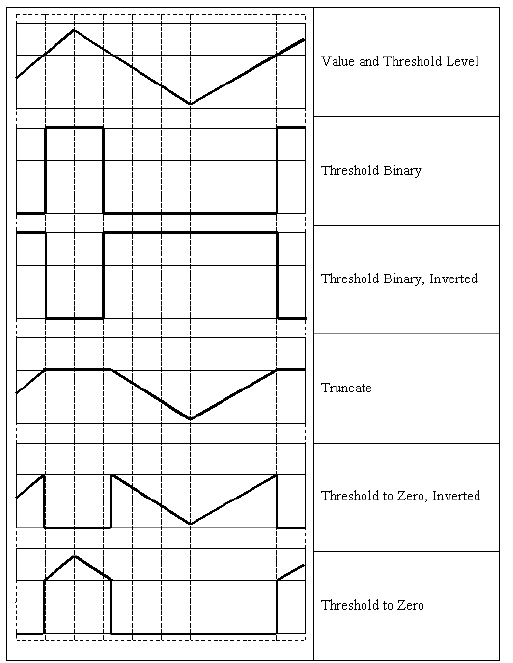
\includegraphics[width=0.5\textwidth]{pics/threshold.png}


\fi

\ifCpp

\cvCppFunc{adaptiveThreshold}
Applies an adaptive threshold to an array.

\cvdefCpp{void adaptiveThreshold( const Mat\& src, Mat\& dst, double maxValue,\par
                        int adaptiveMethod, int thresholdType,\par
                        int blockSize, double C );}
\begin{description}
\cvarg{src}{Source 8-bit single-channel image}
\cvarg{dst}{Destination image; will have the same size and the same type as \texttt{src}}
\cvarg{maxValue}{The non-zero value assigned to the pixels for which the condition is satisfied. See the discussion}
\cvarg{adaptiveMethod}{Adaptive thresholding algorithm to use,
   \texttt{ADAPTIVE\_THRESH\_MEAN\_C} or \texttt{ADAPTIVE\_THRESH\_GAUSSIAN\_C} (see the discussion)}
\cvarg{thresholdType}{Thresholding type; must be one of \texttt{THRESH\_BINARY} or \texttt{THRESH\_BINARY\_INV}}
\cvarg{blockSize}{The size of a pixel neighborhood that is used to calculate a threshold value for the pixel: 3, 5, 7, and so on}
\cvarg{C}{The constant subtracted from the mean or weighted mean (see the discussion); normally, it's positive, but may be zero or negative as well}
\end{description}

The function transforms a grayscale image to a binary image according to the formulas:

\begin{description}
\cvarg{THRESH\_BINARY}{\[ dst(x,y) = \fork{\texttt{maxValue}}{if $src(x,y) > T(x,y)$}{0}{otherwise} \]}
\cvarg{THRESH\_BINARY\_INV}{\[ dst(x,y) = \fork{0}{if $src(x,y) > T(x,y)$}{\texttt{maxValue}}{otherwise} \]}
\end{description}

where $T(x,y)$ is a threshold calculated individually for each pixel.

\begin{enumerate}
    \item
For the method \texttt{ADAPTIVE\_THRESH\_MEAN\_C} the threshold value $T(x,y)$ is the mean of a $\texttt{blockSize} \times \texttt{blockSize}$ neighborhood of $(x, y)$, minus \texttt{C}.
    \item
For the method \texttt{ADAPTIVE\_THRESH\_GAUSSIAN\_C} the threshold value $T(x, y)$ is the weighted sum (i.e. cross-correlation with a Gaussian window) of a $\texttt{blockSize} \times \texttt{blockSize}$ neighborhood of $(x, y)$, minus \texttt{C}. The default sigma (standard deviation) is used for the specified \texttt{blockSize}, see \cvCppCross{getGaussianKernel}.
\end{enumerate}

The function can process the image in-place.

See also: \cvCppCross{threshold}, \cvCppCross{blur}, \cvCppCross{GaussianBlur}


\cvCppFunc{cvtColor}
Converts image from one color space to another

\cvdefCpp{void cvtColor( const Mat\& src, Mat\& dst, int code, int dstCn=0 );}
\begin{description}
\cvarg{src}{The source image, 8-bit unsigned, 16-bit unsigned (\texttt{CV\_16UC...}) or single-precision floating-point}
\cvarg{dst}{The destination image; will have the same size and the same depth as \texttt{src}}
\cvarg{code}{The color space conversion code; see the discussion}
\cvarg{dstCn}{The number of channels in the destination image; if the parameter is 0, the number of the channels will be derived automatically from \texttt{src} and the \texttt{code}}
\end{description}

The function converts the input image from one color
space to another. In the case of transformation to-from RGB color space the ordering of the channels should be specified explicitly (RGB or BGR).

The conventional ranges for R, G and B channel values are:

\begin{itemize}
 \item 0 to 255 for \texttt{CV\_8U} images
 \item 0 to 65535 for \texttt{CV\_16U} images and
 \item 0 to 1 for \texttt{CV\_32F} images.
\end{itemize}

Of course, in the case of linear transformations the range does not matter,
but in the non-linear cases the input RGB image should be normalized to the proper value range in order to get the correct results, e.g. for RGB$\rightarrow$L*u*v* transformation. For example, if you have a 32-bit floating-point image directly converted from 8-bit image without any scaling, then it will have 0..255 value range, instead of the assumed by the function 0..1. So, before calling \texttt{cvtColor}, you need first to scale the image down:
\begin{lstlisting}
img *= 1./255;
cvtColor(img, img, CV_BGR2Luv);
\end{lstlisting}

The function can do the following transformations:

\begin{itemize}
 \item Transformations within RGB space like adding/removing the alpha channel, reversing the channel order, conversion to/from 16-bit RGB color (R5:G6:B5 or R5:G5:B5), as well as conversion to/from grayscale using:
 \[
 \text{RGB[A] to Gray:}\quad Y \leftarrow 0.299 \cdot R + 0.587 \cdot G + 0.114 \cdot B
 \]
 and
 \[
 \text{Gray to RGB[A]:}\quad R \leftarrow Y, G \leftarrow Y, B \leftarrow Y, A \leftarrow 0
 \]

The conversion from a RGB image to gray is done with:
\begin{lstlisting}
cvtColor(src, bwsrc, CV_RGB2GRAY);
\end{lstlisting}

Some more advanced channel reordering can also be done with \cvCppCross{mixChannels}.

 \item RGB $\leftrightarrow$ CIE XYZ.Rec 709 with D65 white point (\texttt{CV\_BGR2XYZ, CV\_RGB2XYZ, CV\_XYZ2BGR, CV\_XYZ2RGB}):
 \[
 \begin{bmatrix}
 X \\
 Y \\
 Z
 \end{bmatrix}
 \leftarrow
 \begin{bmatrix}
0.412453 & 0.357580 & 0.180423\\
0.212671 & 0.715160 & 0.072169\\
0.019334 & 0.119193 & 0.950227
 \end{bmatrix}
 \cdot
 \begin{bmatrix}
 R \\
 G \\
 B
 \end{bmatrix}
 \]
 \[
 \begin{bmatrix}
 R \\
 G \\
 B
 \end{bmatrix}
 \leftarrow
 \begin{bmatrix}
3.240479 & -1.53715 & -0.498535\\
-0.969256 &  1.875991 & 0.041556\\
0.055648 & -0.204043 & 1.057311
 \end{bmatrix}
 \cdot
 \begin{bmatrix}
 X \\
 Y \\
 Z
 \end{bmatrix}
 \]
$X$, $Y$ and $Z$ cover the whole value range (in the case of floating-point images $Z$ may exceed 1).

 \item RGB $\leftrightarrow$ YCrCb JPEG (a.k.a. YCC) (\texttt{CV\_BGR2YCrCb, CV\_RGB2YCrCb, CV\_YCrCb2BGR, CV\_YCrCb2RGB})
 \[ Y \leftarrow 0.299 \cdot R + 0.587 \cdot G + 0.114 \cdot B \]
 \[  Cr \leftarrow (R-Y) \cdot 0.713 + delta \]
 \[  Cb \leftarrow (B-Y) \cdot 0.564 + delta \]
 \[  R \leftarrow Y + 1.403 \cdot (Cr - delta) \]
 \[  G \leftarrow Y - 0.344 \cdot (Cr - delta) - 0.714 \cdot (Cb - delta) \]
 \[  B \leftarrow Y + 1.773 \cdot (Cb - delta) \]
where
 \[
  delta = \left\{
  \begin{array}{l l}
  128 & \mbox{for 8-bit images}\\
  32768 & \mbox{for 16-bit images}\\
  0.5 & \mbox{for floating-point images}
  \end{array} \right.
 \]
Y, Cr and Cb cover the whole value range.

 \item RGB $\leftrightarrow$ HSV (\texttt{CV\_BGR2HSV, CV\_RGB2HSV, CV\_HSV2BGR, CV\_HSV2RGB})
  in the case of 8-bit and 16-bit images
  R, G and B are converted to floating-point format and scaled to fit the 0 to 1 range
  \[ V \leftarrow max(R,G,B) \]

\[ S \leftarrow \fork{\frac{V-min(R,G,B)}{V}}{if $V \neq 0$}{0}{otherwise} \]
\[ H \leftarrow \forkthree
{{60(G - B)}/{S}}{if $V=R$}
{{120+60(B - R)}/{S}}{if $V=G$}
{{240+60(R - G)}/{S}}{if $V=B$} \]
if $H<0$ then $H \leftarrow H+360$

On output $0 \leq V \leq 1$, $0 \leq S \leq 1$, $0 \leq H \leq 360$.

The values are then converted to the destination data type:
\begin{description}
\item[8-bit images]
\[ V \leftarrow 255 V, S \leftarrow 255 S, H \leftarrow H/2 \text{(to fit to 0 to 255)} \]
\item[16-bit images (currently not supported)]
\[ V <- 65535 V, S <- 65535 S, H <- H \]
\item[32-bit images]
H, S, V are left as is
\end{description}

 \item RGB $\leftrightarrow$ HLS (\texttt{CV\_BGR2HLS, CV\_RGB2HLS, CV\_HLS2BGR, CV\_HLS2RGB}).
  in the case of 8-bit and 16-bit images
  R, G and B are converted to floating-point format and scaled to fit the 0 to 1 range.
  \[ V_{max} \leftarrow {max}(R,G,B) \]
  \[ V_{min} \leftarrow {min}(R,G,B) \]
  \[ L \leftarrow \frac{V_{max} - V_{min}}{2} \]
  \[ S \leftarrow \fork
    {\frac{V_{max} - V_{min}}{V_{max} + V_{min}}}{if $L < 0.5$}
    {\frac{V_{max} - V_{min}}{2 - (V_{max} + V_{min})}}{if $L \ge 0.5$} \]
  \[ H \leftarrow \forkthree
  {{60(G - B)}/{S}}{if $V_{max}=R$}
  {{120+60(B - R)}/{S}}{if $V_{max}=G$}
  {{240+60(R - G)}/{S}}{if $V_{max}=B$} \]
  if $H<0$ then $H \leftarrow H+360$
On output $0 \leq V \leq 1$, $0 \leq S \leq 1$, $0 \leq H \leq 360$.

The values are then converted to the destination data type:
\begin{description}
\item[8-bit images]
\[ V \leftarrow 255\cdot V, S \leftarrow 255\cdot S, H \leftarrow H/2\; \text{(to fit to 0 to 255)} \]
\item[16-bit images (currently not supported)]
\[ V <- 65535\cdot V, S <- 65535\cdot S, H <- H \]
\item[32-bit images]
H, S, V are left as is
\end{description}

 \item RGB $\leftrightarrow$ CIE L*a*b* (\texttt{CV\_BGR2Lab, CV\_RGB2Lab, CV\_Lab2BGR, CV\_Lab2RGB})
  in the case of 8-bit and 16-bit images
  R, G and B are converted to floating-point format and scaled to fit the 0 to 1 range
\[ \vecthree{X}{Y}{Z} \leftarrow \vecthreethree
{0.412453}{0.357580}{0.180423}
{0.212671}{0.715160}{0.072169}
{0.019334}{0.119193}{0.950227}
\cdot
\vecthree{R}{G}{B} \]
\[ X \leftarrow X/X_n, \text{where} X_n = 0.950456 \]
\[ Z \leftarrow Z/Z_n, \text{where} Z_n = 1.088754 \]
\[ L \leftarrow \fork
{116*Y^{1/3}-16}{for $Y>0.008856$}
{903.3*Y}{for $Y \le 0.008856$} \]
\[ a \leftarrow 500 (f(X)-f(Y)) + delta \]
\[ b \leftarrow 200 (f(Y)-f(Z)) + delta \]
where
\[f(t)=\fork
{t^{1/3}}{for $t>0.008856$}
{7.787 t+16/116}{for $t\leq 0.008856$} \]
and
\[ delta = \fork{128}{for 8-bit images}{0}{for floating-point images} \]
On output $0 \leq L \leq 100$, $-127 \leq a \leq 127$, $-127 \leq b \leq 127$

The values are then converted to the destination data type:
\begin{description}
\item[8-bit images]
\[L \leftarrow L*255/100,\; a \leftarrow a + 128,\; b \leftarrow b + 128\]
\item[16-bit images] currently not supported
\item[32-bit images]
L, a, b are left as is
\end{description}

 \item RGB $\leftrightarrow$ CIE L*u*v* (\texttt{CV\_BGR2Luv, CV\_RGB2Luv, CV\_Luv2BGR, CV\_Luv2RGB})
  in the case of 8-bit and 16-bit images
  R, G and B are converted to floating-point format and scaled to fit 0 to 1 range
  \[ \vecthree{X}{Y}{Z} \leftarrow \vecthreethree
{0.412453}{0.357580}{0.180423}
{0.212671}{0.715160}{0.072169}
{0.019334}{0.119193}{0.950227}
\cdot
\vecthree{R}{G}{B} \]
\[ L \leftarrow \fork
{116 Y^{1/3}}{for $Y>0.008856$}
{903.3 Y}{for $Y\leq 0.008856$} \]
\[ u' \leftarrow 4*X/(X + 15*Y + 3 Z) \]
\[ v' \leftarrow 9*Y/(X + 15*Y + 3 Z) \]
\[ u \leftarrow 13*L*(u' - u_n) \quad \text{where} \quad u_n=0.19793943 \]
\[ v \leftarrow 13*L*(v' - v_n) \quad \text{where} \quad v_n=0.46831096 \]
On output $0 \leq L \leq 100$, $-134 \leq u \leq 220$, $-140 \leq v \leq 122$.

The values are then converted to the destination data type:
\begin{description}
\item[8-bit images]
\[L \leftarrow 255/100 L,\; u \leftarrow 255/354 (u + 134),\; v \leftarrow 255/256 (v + 140) \]
\item[16-bit images] currently not supported
\item[32-bit images] L, u, v are left as is
\end{description}

The above formulas for converting RGB to/from various color spaces have been taken from multiple sources on Web, primarily from the Charles Poynton site \url{http://www.poynton.com/ColorFAQ.html}

 \item Bayer $\rightarrow$ RGB (\texttt{CV\_BayerBG2BGR, CV\_BayerGB2BGR, CV\_BayerRG2BGR, CV\_BayerGR2BGR, CV\_BayerBG2RGB, CV\_BayerGB2RGB, CV\_BayerRG2RGB, CV\_BayerGR2RGB}) The Bayer pattern is widely used in CCD and CMOS cameras. It allows one to get color pictures from a single plane where R,G and B pixels (sensors of a particular component) are interleaved like this:

\[
\newcommand{\Rcell}{\color{red}R}
\newcommand{\Gcell}{\color{green}G}
\newcommand{\Bcell}{\color{blue}B}
\definecolor{BackGray}{rgb}{0.8,0.8,0.8}
\begin{array}{ c c c c c }
\Rcell&\Gcell&\Rcell&\Gcell&\Rcell\\
\Gcell&\colorbox{BackGray}{\Bcell}&\colorbox{BackGray}{\Gcell}&\Bcell&\Gcell\\
\Rcell&\Gcell&\Rcell&\Gcell&\Rcell\\
\Gcell&\Bcell&\Gcell&\Bcell&\Gcell\\
\Rcell&\Gcell&\Rcell&\Gcell&\Rcell
\end{array}
\]

The output RGB components of a pixel are interpolated from 1, 2 or
4 neighbors of the pixel having the same color. There are several
modifications of the above pattern that can be achieved by shifting
the pattern one pixel left and/or one pixel up. The two letters
$C_1$ and $C_2$
in the conversion constants
\texttt{CV\_Bayer} $ C_1 C_2 $ \texttt{2BGR}
and
\texttt{CV\_Bayer} $ C_1 C_2 $ \texttt{2RGB}
indicate the particular pattern
type - these are components from the second row, second and third
columns, respectively. For example, the above pattern has very
popular "BG" type.
\end{itemize}



\cvCppFunc{distanceTransform}
Calculates the distance to the closest zero pixel for each pixel of the source image.

\cvdefCpp{void distanceTransform( const Mat\& src, Mat\& dst,\par
                        int distanceType, int maskSize );\newline
void distanceTransform( const Mat\& src, Mat\& dst, Mat\& labels,\par
                        int distanceType, int maskSize );}
\begin{description}
\cvarg{src}{8-bit, single-channel (binary) source image}
\cvarg{dst}{Output image with calculated distances; will be 32-bit floating-point, single-channel image of the same size as \texttt{src}}
\cvarg{distanceType}{Type of distance; can be \texttt{CV\_DIST\_L1, CV\_DIST\_L2} or \texttt{CV\_DIST\_C}}
\cvarg{maskSize}{Size of the distance transform mask; can be 3, 5 or \texttt{CV\_DIST\_MASK\_PRECISE} (the latter option is only supported by the first of the functions). In the case of \texttt{CV\_DIST\_L1} or \texttt{CV\_DIST\_C} distance type the parameter is forced to 3, because a $3\times 3$ mask gives the same result as a $5\times 5$ or any larger aperture.}
\cvarg{labels}{The optional output 2d array of labels - the discrete Voronoi diagram; will have type \texttt{CV\_32SC1} and the same size as \texttt{src}. See the discussion}
\end{description}

The functions \texttt{distanceTransform} calculate the approximate or precise
distance from every binary image pixel to the nearest zero pixel.
(for zero image pixels the distance will obviously be zero).

When \texttt{maskSize == CV\_DIST\_MASK\_PRECISE} and \texttt{distanceType == CV\_DIST\_L2}, the function runs the algorithm described in \cite{Felzenszwalb04}.

In other cases the algorithm \cite{Borgefors86} is used, that is,
for pixel the function finds the shortest path to the nearest zero pixel
consisting of basic shifts: horizontal,
vertical, diagonal or knight's move (the latest is available for a
$5\times 5$ mask). The overall distance is calculated as a sum of these
basic distances. Because the distance function should be symmetric,
all of the horizontal and vertical shifts must have the same cost (that
is denoted as \texttt{a}), all the diagonal shifts must have the
same cost (denoted \texttt{b}), and all knight's moves must have
the same cost (denoted \texttt{c}). For \texttt{CV\_DIST\_C} and
\texttt{CV\_DIST\_L1} types the distance is calculated precisely,
whereas for \texttt{CV\_DIST\_L2} (Euclidian distance) the distance
can be calculated only with some relative error (a $5\times 5$ mask
gives more accurate results). For \texttt{a}, \texttt{b} and \texttt{c}
OpenCV uses the values suggested in the original paper:


\begin{tabular}{| c | c | c |}
\hline
\texttt{CV\_DIST\_C}  & $(3\times 3)$ & a = 1, b = 1\\ \hline
\texttt{CV\_DIST\_L1} & $(3\times 3)$ & a = 1, b = 2\\ \hline
\texttt{CV\_DIST\_L2} & $(3\times 3)$ & a=0.955, b=1.3693\\ \hline
\texttt{CV\_DIST\_L2} & $(5\times 5)$ & a=1, b=1.4, c=2.1969\\ \hline
\end{tabular}


Typically, for a fast, coarse distance estimation \texttt{CV\_DIST\_L2},
a $3\times 3$ mask is used, and for a more accurate distance estimation
\texttt{CV\_DIST\_L2}, a $5\times 5$ mask or the precise algorithm is used.
Note that both the precise and the approximate algorithms are linear on the number of pixels.

The second variant of the function does not only compute the minimum distance for each pixel $(x, y)$,
but it also identifies the nearest the nearest connected
component consisting of zero pixels. Index of the component is stored in $\texttt{labels}(x, y)$.
The connected components of zero pixels are also found and marked by the function.

In this mode the complexity is still linear.
That is, the function provides a very fast way to compute Voronoi diagram for the binary image.
Currently, this second variant can only use the approximate distance transform algorithm.


\cvCppFunc{floodFill}
Fills a connected component with the given color.

\cvdefCpp{int floodFill( Mat\& image,\par
               Point seed, Scalar newVal, Rect* rect=0,\par
               Scalar loDiff=Scalar(), Scalar upDiff=Scalar(),\par
               int flags=4 );\newline
int floodFill( Mat\& image, Mat\& mask,\par
               Point seed, Scalar newVal, Rect* rect=0,\par
               Scalar loDiff=Scalar(), Scalar upDiff=Scalar(),\par
               int flags=4 );}
\begin{description}
\cvarg{image}{Input/output 1- or 3-channel, 8-bit or floating-point image. It is modified by the function unless the \texttt{FLOODFILL\_MASK\_ONLY} flag is set (in the second variant of the function; see below)}
\cvarg{mask}{(For the second function only) Operation mask, should be a single-channel 8-bit image, 2 pixels wider and 2 pixels taller. The function uses and updates the mask, so the user takes responsibility of initializing the \texttt{mask} content. Flood-filling can't go across non-zero pixels in the mask, for example, an edge detector output can be used as a mask to stop filling at edges. It is possible to use the same mask in multiple calls to the function to make sure the filled area do not overlap. \textbf{Note}: because the mask is larger than the filled image, a pixel $(x, y)$ in \texttt{image} will correspond to the pixel $(x+1, y+1)$ in the \texttt{mask}}
\cvarg{seed}{The starting point}
\cvarg{newVal}{New value of the repainted domain pixels}
\cvarg{loDiff}{Maximal lower brightness/color difference between the currently observed pixel and one of its neighbors belonging to the component, or a seed pixel being added to the component}
\cvarg{upDiff}{Maximal upper brightness/color difference between the currently observed pixel and one of its neighbors belonging to the component, or a seed pixel being added to the component}
\cvarg{rect}{The optional output parameter that the function sets to the minimum bounding rectangle of the repainted domain}
\cvarg{flags}{The operation flags. Lower bits contain connectivity value, 4 (by default) or 8, used within the function. Connectivity determines which neighbors of a pixel are considered. Upper bits can be 0 or a combination of the following flags:
\begin{description}
  \cvarg{FLOODFILL\_FIXED\_RANGE}{if set, the difference between the current pixel and seed pixel is considered, otherwise the difference between neighbor pixels is considered (i.e. the range is floating)}
  \cvarg{FLOODFILL\_MASK\_ONLY}{(for the second variant only) if set, the function does not change the image (\texttt{newVal} is ignored), but fills the mask}
\end{description}}
\end{description}

The functions \texttt{floodFill} fill a connected component starting from the seed point with the specified color. The connectivity is determined by the color/brightness closeness of the neighbor pixels. The pixel at $(x,y)$ is considered to belong to the repainted domain if:

\begin{description}

\item[grayscale image, floating range] \[
\texttt{src}(x',y')-\texttt{loDiff} \leq \texttt{src}(x,y) \leq \texttt{src}(x',y')+\texttt{upDiff} \]

\item[grayscale image, fixed range] \[
\texttt{src}(\texttt{seed}.x,\texttt{seed}.y)-\texttt{loDiff}\leq \texttt{src}(x,y) \leq \texttt{src}(\texttt{seed}.x,\texttt{seed}.y)+\texttt{upDiff} \]

\item[color image, floating range]
\[ \texttt{src}(x',y')_r-\texttt{loDiff}_r\leq \texttt{src}(x,y)_r\leq \texttt{src}(x',y')_r+\texttt{upDiff}_r \]
\[ \texttt{src}(x',y')_g-\texttt{loDiff}_g\leq \texttt{src}(x,y)_g\leq \texttt{src}(x',y')_g+\texttt{upDiff}_g \]
\[ \texttt{src}(x',y')_b-\texttt{loDiff}_b\leq \texttt{src}(x,y)_b\leq \texttt{src}(x',y')_b+\texttt{upDiff}_b \]

\item[color image, fixed range]
\[ \texttt{src}(\texttt{seed}.x,\texttt{seed}.y)_r-\texttt{loDiff}_r\leq \texttt{src}(x,y)_r\leq \texttt{src}(\texttt{seed}.x,\texttt{seed}.y)_r+\texttt{upDiff}_r \]
\[ \texttt{src}(\texttt{seed}.x,\texttt{seed}.y)_g-\texttt{loDiff}_g\leq \texttt{src}(x,y)_g\leq \texttt{src}(\texttt{seed}.x,\texttt{seed}.y)_g+\texttt{upDiff}_g \]
\[ \texttt{src}(\texttt{seed}.x,\texttt{seed}.y)_b-\texttt{loDiff}_b\leq \texttt{src}(x,y)_b\leq \texttt{src}(\texttt{seed}.x,\texttt{seed}.y)_b+\texttt{upDiff}_b \]
\end{description}

where $src(x',y')$ is the value of one of pixel neighbors that is already known to belong to the component. That is, to be added to the connected component, a pixel's color/brightness should be close enough to the:
\begin{itemize}
  \item color/brightness of one of its neighbors that are already referred to the connected component in the case of floating range
  \item color/brightness of the seed point in the case of fixed range.
\end{itemize}

By using these functions you can either mark a connected component with the specified color in-place, or build a mask and then extract the contour or copy the region to another image etc. Various modes of the function are demonstrated in \texttt{floodfill.c} sample.

See also: \cvCppCross{findContours}


\cvCppFunc{inpaint}
Inpaints the selected region in the image.

\cvdefCpp{void inpaint( const Mat\& src, const Mat\& inpaintMask,\par
              Mat\& dst, double inpaintRadius, int flags );}

\begin{description}
\cvarg{src}{The input 8-bit 1-channel or 3-channel image.}
\cvarg{inpaintMask}{The inpainting mask, 8-bit 1-channel image. Non-zero pixels indicate the area that needs to be inpainted.}
\cvarg{dst}{The output image; will have the same size and the same type as \texttt{src}}
\cvarg{inpaintRadius}{The radius of a circlular neighborhood of each point inpainted that is considered by the algorithm.}
\cvarg{flags}{The inpainting method, one of the following:
\begin{description}
\cvarg{INPAINT\_NS}{Navier-Stokes based method.}
\cvarg{INPAINT\_TELEA}{The method by Alexandru Telea \cite{Telea04}}
\end{description}}
\end{description}

The function reconstructs the selected image area from the pixel near the area boundary. The function may be used to remove dust and scratches from a scanned photo, or to remove undesirable objects from still images or video. See \url{http://en.wikipedia.org/wiki/Inpainting} for more details.


\cvCppFunc{integral}
Calculates the integral of an image.

\cvdefCpp{void integral( const Mat\& image, Mat\& sum, int sdepth=-1 );\newline
void integral( const Mat\& image, Mat\& sum, Mat\& sqsum, int sdepth=-1 );\newline
void integral( const Mat\& image, Mat\& sum, \par Mat\& sqsum, Mat\& tilted, int sdepth=-1 );}
\begin{description}
\cvarg{image}{The source image, $W \times H$, 8-bit or floating-point (32f or 64f)}
\cvarg{sum}{The integral image, $(W+1)\times (H+1)$, 32-bit integer or floating-point (32f or 64f)}
\cvarg{sqsum}{The integral image for squared pixel values, $(W+1)\times (H+1)$, double precision floating-point (64f)}
\cvarg{tilted}{The integral for the image rotated by 45 degrees, $(W+1)\times (H+1)$, the same data type as \texttt{sum}}
\cvarg{sdepth}{The desired depth of the integral and the tilted integral images, \texttt{CV\_32S},  \texttt{CV\_32F} or \texttt{CV\_64F}}
\end{description}

The functions \texttt{integral} calculate one or more integral images for the source image as following:

\[
\texttt{sum}(X,Y) = \sum_{x<X,y<Y} \texttt{image}(x,y)
\]

\[
\texttt{sqsum}(X,Y) = \sum_{x<X,y<Y} \texttt{image}(x,y)^2
\]

\[
\texttt{tilted}(X,Y) = \sum_{y<Y,abs(x-X)<y} \texttt{image}(x,y)
\]

Using these integral images, one may calculate sum, mean and standard deviation over a specific up-right or rotated rectangular region of the image in a constant time, for example:

\[
\sum_{x_1\leq x < x_2, \, y_1 \leq y < y_2} \texttt{image}(x,y) = \texttt{sum}(x_2,y_2)-\texttt{sum}(x_1,y_2)-\texttt{sum}(x_2,y_1)+\texttt{sum}(x_1,x_1)
\]

It makes possible to do a fast blurring or fast block correlation with variable window size, for example. In the case of multi-channel images, sums for each channel are accumulated independently.


\cvCppFunc{threshold}
Applies a fixed-level threshold to each array element

\cvdefCpp{double threshold( const Mat\& src, Mat\& dst, double thresh,\par
                  double maxVal, int thresholdType );}
\begin{description}
\cvarg{src}{Source array (single-channel, 8-bit of 32-bit floating point)}
\cvarg{dst}{Destination array; will have the same size and the same type as \texttt{src}}
\cvarg{thresh}{Threshold value}
\cvarg{maxVal}{Maximum value to use with \texttt{THRESH\_BINARY} and \texttt{THRESH\_BINARY\_INV} thresholding types}
\cvarg{thresholdType}{Thresholding type (see the discussion)}
\end{description}

The function applies fixed-level thresholding
to a single-channel array. The function is typically used to get a
bi-level (binary) image out of a grayscale image (\cvCppCross{compare} could
be also used for this purpose) or for removing a noise, i.e. filtering
out pixels with too small or too large values. There are several
types of thresholding that the function supports that are determined by
\texttt{thresholdType}:

\begin{description}
\cvarg{THRESH\_BINARY}{\[ \texttt{dst}(x,y) = \fork{\texttt{maxVal}}{if $\texttt{src}(x,y) > \texttt{thresh}$}{0}{otherwise} \]}
\cvarg{THRESH\_BINARY\_INV}{\[ \texttt{dst}(x,y) = \fork{0}{if $\texttt{src}(x,y) > \texttt{thresh}$}{\texttt{maxVal}}{otherwise} \]}
\cvarg{THRESH\_TRUNC}{\[ \texttt{dst}(x,y) = \fork{\texttt{threshold}}{if $\texttt{src}(x,y) > \texttt{thresh}$}{\texttt{src}(x,y)}{otherwise} \]}
\cvarg{THRESH\_TOZERO}{\[ \texttt{dst}(x,y) = \fork{\texttt{src}(x,y)}{if $\texttt{src}(x,y) > \texttt{thresh}$}{0}{otherwise} \]}
\cvarg{THRESH\_TOZERO\_INV}{\[ \texttt{dst}(x,y) = \fork{0}{if $\texttt{src}(x,y) > \texttt{thresh}$}{\texttt{src}(x,y)}{otherwise} \]}
\end{description}

Also, the special value \texttt{THRESH\_OTSU} may be combined with
one of the above values. In this case the function determines the optimal threshold
value using Otsu's algorithm and uses it instead of the specified \texttt{thresh}.
The function returns the computed threshold value.
Currently, Otsu's method is implemented only for 8-bit images.

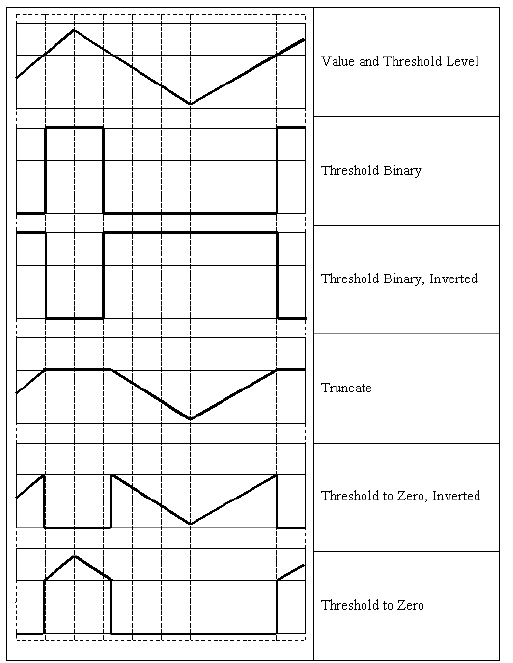
\includegraphics[width=0.5\textwidth]{pics/threshold.png}

See also: \cvCppCross{adaptiveThreshold}, \cvCppCross{findContours}, \cvCppCross{compare}, \cvCppCross{min}, \cvCppCross{max}

\cvCppFunc{watershed}
Does marker-based image segmentation using watershed algrorithm

\cvdefCpp{void watershed( const Mat\& image, Mat\& markers );}
\begin{description}
\cvarg{image}{The input 8-bit 3-channel image.} 
\cvarg{markers}{The input/output 32-bit single-channel image (map) of markers. It should have the same size as \texttt{image}}
\end{description}

The function implements one of the variants
of watershed, non-parametric marker-based segmentation algorithm,
described in \cite{Meyer92}. Before passing the image to the
function, user has to outline roughly the desired regions in the image
\texttt{markers} with positive ($>0$) indices, i.e. every region is
represented as one or more connected components with the pixel values
1, 2, 3 etc (such markers can be retrieved from a binary mask
using \cvCppCross{findContours}and \cvCppCross{drawContours}, see \texttt{watershed.cpp} demo).
The markers will be "seeds" of the future image
regions. All the other pixels in \texttt{markers}, which relation to the
outlined regions is not known and should be defined by the algorithm,
should be set to 0's. On the output of the function, each pixel in
markers is set to one of values of the "seed" components, or to -1 at
boundaries between the regions.

Note, that it is not necessary that every two neighbor connected
components are separated by a watershed boundary (-1's pixels), for
example, in case when such tangent components exist in the initial
marker image. Visual demonstration and usage example of the function
can be found in OpenCV samples directory; see \texttt{watershed.cpp} demo.

See also: \cvCppCross{findContours}

\fi
